\chapter{绪论}
\chaptermark{绪论}
\section{课题研究目的和意义}

刀具作为数控加工的主要工具,其磨损状态对于被加工产品的质量、整体加工的成本、使用效率和能耗有非常重要的影响。当加工零件时,如果刀具的磨损已经达到失效阈值或者产生了其他缺陷,加工时零件表面温度可能升高,刀具切削也会发生振颤,这都会危及加工件的质量甚至整个机床的安全生产,带来较大的损失。根据数据\cite{kegg1984one,kurada1997review}表明,7\%-20\%的机床停机都是由于刀具损坏造成,其对企业带来了很大的损失。但是出于成本考量,过于保守的估计刀具使得刀具被提前更换,即提高了加工的生产成本,影响产品的竞争力,也会干扰正常的加工过程,使得加工时长加长,很大程度影响最终生产力和加工产品在成本的竞争力。因此,如何准确而稳健的监测及预报刀具磨损量成为了学术界和工业界的关注重点。

基于以上的背景,很多研究都开始从事刀具磨损量的监测上。由于前刀面不与加工工件接触,而后刀面则直接切削加工工件,刀具磨损量往往选择刀具的后刀面磨损量作为主要指标。通过准确的获得刀具后刀面磨损量的信息,加工者就可以评估刀具是否适合更换以及为刀具的合理选用提供决策。然而,刀具磨损量监测仍然面临着较大的挑战。通过观察切削时振动、声音和切削非常依赖专家系统和先验知识,比较偏玄学,在稳健性上缺少应用基础;基于数理统计的方法和静态Taylor公式\cite{marksberry2008comprehensive}的结合则忽视了不同刀具的个题差异性和刀具磨损的退化轨迹;基于经典机器学习的方法能够给出磨损量的点估计,然而在实际应用时也非常依赖对于样本数据的分布判断,同时为了保证模型的泛化性,往往需要充足的数据进行训练以及评估泛化性能,对于变化工况的情形适应力较差\cite{si2017data}。同时几乎没有研究关注在针对刀具未来磨损量趋势预测进行建模分析,而针对未来的趋势预报对于提前预警来说具有非常重要的意义。

造成以上的问题在于,刀具磨损退化过程十分复杂并且具有较强的非线性。在常见的加工中,工件和刀具往往发生了物理、化学变化并且伴有较为明显的热力学影响,这都导致刀具磨损退化具有显著的随机性。同时不同批次的刀具之间也存在着一定的差异性,会对预报产生影响。另外,切削参数、工件材料也会对整个加工过程产生不可忽视的影响\cite{liang2017experimental}。因此,必须考虑模型泛化性能的前提下进行建模,直接检测加工时信号表征刀具磨损状态,从而进行刀具磨损状态的识别。同时基于多工况下特征共享设计,使得网络能够有效的识别不同工况下的磨损量状态,从而实现基于加工信号的多工况下刀具磨损量监测。

针对以上问题,本研究以铣削加工作为研究对象,通过铣削实验获得刀具磨损量随着加工循环的数据,利用\gls{cnn_zh}为基础,建立从多维加工信号到刀具磨损量映射的深度学习模型,针对刀具磨损量进行监测。利用以\gls{lstm_zh}单元为基础的\gls{rnn_zh}模型,针对刀具磨损量退化轨迹进行建模,从而得到历史磨损量和未来磨损量值之间的关联,从而完成针对未来磨损量的趋势预报。针对\gls{cnn_zh}模型进行可视化和可解释分析,为刀具磨损监测提出科学参考,并且验证多工况下刀具磨损检测的合理性以及迁移学习的科学性。本研究对于在加工过程中保证产品质量、提高生产力、提高产品竞争力,对于智能化制造具有非常重要的意义。

\section{国内外研究现状}

\subsection{刀具磨损量监测研究现状}

刀具后刀面磨损量可以很好的显示刀具目前的切削状态。在加工工件时,后刀面持续接触、切削工件使得后刀面逐渐钝化,使得刀具切削性能变差,可靠性和稳定性降低。在切削性能下降到某个程度后,继续切削将会引起工件的质量缺陷、机床的颤振甚至最终安全事故。监测不同时间的刀具磨损状态,建立其退化失效模型。目前,刀具磨损状态的监测可以大致分为直接和间接两种。

直接法通过光学或者其他仪器直接测量后刀面的磨损量。比较常见的有电流、激光和图像的方法直接测量刀具磨损量。Jeon\cite{jeon1988optical}使用图像处理的方法直接测量了后刀面磨损量,其分辨率可以达到0.1mm。其他的还有诸如激光和声信号\cite{giardini1996neural,shahabi2009cycle,xiong2011cutting},它们都能精准地测量的刀具磨损量。但是由于实际加工工件时,因为遮挡或者切削液和切屑干扰问题,实时获得刀具信号往往很困难,一般都需要中断加工才能进行光学测量。同时由于稳定性和精确度地要求,这些设备都需要特殊的布置。所以在连续加工的情形下,使用间接法进行刀具后刀面磨损量的测量是目前比较主要的方法。

间接法通过加工时的三轴力\cite{dimla2000line,saglam2003tool}、三轴加速度\cite{polini2007monitoring,yesilyurt2007tool,lin1996tool,fu2011cutting,zhang2008tool}、声发射信号\cite{dimla2000sensor}、主轴电流信号\cite{kim2011fuzzy}、机床功率\cite{drouillet2016tool}等信号评估当前工件磨损状态,往往使用专家系统或者一些自适应地方法选择某些指标,提取与刀具磨损具有显著相关性的特征,根据这些特征完成对于刀具磨损状态的识别,进而监测刀具磨损量。Wong\cite{wong2004experimental}等人和Dimla\cite{dimla2000sensor}在它们的文章中都明确表达了,通过传感器的信号,刀具的状态是能够被预测的。这使得在线实时监测刀具状态变得可能。对于建立特征到刀具磨损状态而言,研究者们使用了各式各样的算法,并且都取得了一定的成果。Huang\cite{huang2000neural}使用神经网络的方法研究刀具失效问题,其精度达到了90.7\%。Rizal等人\cite{rizal2013online}和Yingxue\cite{yao1999tool}使用了一种自适应的模糊神经网络算法来在线预测刀具磨损量。Benkedjouh等人\cite{benkedjouh2015health}使用了\gls{svm_zh}的方法通过某些高级特征来估计刀具的磨损等级。Chen\cite{chen2005artificial}使用了一个带有全连接层的\gls{ann_zh}来预测刀具磨损量,其误差较小。同样基于神经网络的方法也被Ezugwu \cite{ezugwu1995tool}, Ghosh \cite{ghosh2007estimation}, Palanisamy \cite{palanisamy2008prediction}, Quiza \cite{quiza2008comparing} 和 Sick \cite{sick2002line}采用。

然而常见的间接法都很依赖于对于特征的人工选择,中国科学院大学曾广圣使用多信息和多融合技术\cite{曾广圣2017基于多信息和多模型融合的刀具磨损预测性评估的方法研究}在其硕士论文中提出了超过120个不同的信号特征,并且对比了它们对于最终刀具磨损特征的影响系数。其文章指出,刀具磨损状态和力、振动和声发射信号具有一定程度的关系,同时如何从信号中提取特征也会影响最终模型预测的精度。

同时,由于加工时工况在不断变化,对于多工况下的刀具磨损量监测,对于大量不同的工况都建立相应的模型非常耗费成本,同时由于大部分的方法都很依赖数据的量级,对于大量数据进行专家系统的识别、筛选以及建立磨损量关系必然耗费大量的时间和精力。一般来说,对于某些样本较少的工况,这种推倒重来的方法显得尤为不切实际。如何对于不同工况下信号特征进行复用,其成为了解决多工况下刀具磨损量监测的一个难题。目前对于多个工况下的刀具磨损量识别也比较少。

随着人工智能技术的发展,以\gls{cnn_zh}为代表的深度学习方法逐渐地被应用于刀具磨损状态监测和预报上,通过有监督学习的方式训练\gls{cnn_zh},利用卷积滤波器对于信号中的特征进行捕捉,利用\gls{mlp_zh}针对特征进行逐层抽象并滤去冗余信息,利用全连接层给建立抽象层上高级特征与刀具磨损状态的关系,进而得到以加工信号为输入,刀具磨损量为输出的深度学习模型。Zhao等人\cite{zhao2019deep}总结了深度学习对于机器健康诊断的应用。Jia等人\cite{jia2016deep}使用深度网络的方法对于磨削时的大数据信息进行了失效诊断,并且取得了较好的结果。这种基于深度学习的方法在监测的精度上相对于传统方法有着较大的超越,也是目前较为热门的一个前沿。

同时,以迁移学习\cite{pan2010survey}为代表的深度学习技术允许模型能够在不同的工况下重用不同条件下的特征,并且准确的给出对应的标签。这种方法使得深度学习模型能够在多工况下实现对于不同工况下刀具磨损的识别。

\subsection{刀具磨损量预报研究现状}

目前由于磨损量监测的精度不甚高,在需要进一步支持的预报领域仅有非常少的研究。对于刀具预报而言,由于其对于加工生产具有预警作用,故受到了很多关注。近些年来国内外学者针对机械中的预报问题的研究主要是Markov链和其变体的模型\cite{wang2002hidden,karandikar2014tool,ertunc2001decision}。而本文将会提出一种全新的基于\gls{lstm_zh}的\gls{rnn_zh}模型,极高精度并且强泛化地给出刀具磨损量的未来趋势变化。

基于Markov链方法都认为下一个时刻的刀具退化轨迹与上一个时刻的刀具退化具有强烈的关系,针对马尔科夫模型的改进也考虑了更多时长下的刀具磨损量的值。并且这些方法都得到了一个较好的退化轨迹模型,然而其针对刀具磨损过于简化,在模型建立的时候遗漏了很多的信息并且带有主观感觉,并没有反应刀具磨损量和历史磨损量存在的真实关系。考虑更多时刻的刀具磨损量的依据也不可靠,没有给出数据和物理依据,其给出的预报精度也不是很高。

Caggiano等人\cite{caggiano2018multiple}则使用了多个传感器监测的数据来驱动一个简单的人工神经网络,来预测复合材料加工的时候的刀具磨损量。而这种预报的方法选取的磨损量的样本较少,不具有普适性和通用性,同时这种方法需要大量的历史数据,在早期切削的时候,模型由于没有足够的历史磨损量数据无法使用。在早期切削的时候,模型首先就没有启动需要的数据。同时在实际加工的过程中不可能实时的卸载刀具直接测量磨损量,对于加工的实时性和实用性提出了很大的挑战。上面所说的这些方法往往是离线的算法,并没有办法进行扩展和在线纠正。Martinov等人\cite{martinov2015real}通过监测信号的特征状态实现了针对刀具磨损状态的预测,其仅仅是预测出了目前的刀具的磨损状态,既没有给出具体的磨损量的值也没有给出刀具在下一个时刻的磨损量变化情况。其结果比较笼统而模糊,并没有反应刀具磨损量的退化情况,只是离散地给出了刀具状态的目前状态。在实际加工的时候参考意义不大。Martinova等人\cite{martinova2012diagnostics}通过实时的监测自反馈从而完成了诊断和预报的过程。其针对磨损量的预报仅仅是对监测数据在时间轴做一个线性的延拓,而刀具退化往往是一个非线性过程,并伴有平台期的出现。使用这种方法在刀具退化轨迹的非线性段预测,其误差是非常巨大的。

而基于\gls{rnn_zh}的方法使用细胞链的状态响应某一段时间内刀具磨损量的变化,综合考虑了历史所有时刻的磨损量的值,并得到下一个未来时段的刀具磨损量。通过增加或者减小细胞的个数,可以灵活地完成短期和长期的预报任务。短期预报同时也能在切削早期启动,避免了早期因为历史数据的个数限制导致的无法正常工作的情况。同时通过监测磨损量值的方法,可以对未来预测值进行在线修正,极大的增强了方法在实际生产应用的可靠性和可操作性。这种方法通过细胞状态内的门径机制表现了当前磨损状态和历史磨损状态的关联关系,通过数据驱动更好地反映了刀具退化轨迹,其精度远远超过现有的预报方法。

由于基于\gls{lstm_zh}的\gls{rnn_zh}模型能够很好的建立刀具磨损退化轨迹,同时通过变更编码器和解码器的细胞个数能够灵活的完成对于不同时长内的未来趋势预报,所以基于\gls{rnn_zh}的未来趋势预报是目前刀具磨损在线预报的一个非常优良的方法。

\section{刀具磨损监测和预报问题以及其发展趋势}

综上所述,研究内容的难点和发展趋势可以总结如下:

\begin{enumerate}
	\item 对于信号的特征选取、识别、筛选成为了影响刀具磨损监测问题的关键。在传统方法中,这往往需要研究人员事无巨细并且敏锐地识别出信号中的关键部分。同时也对研究人员的先验知识和奇淫技巧提出了挑战。这种方法往往会使得特征产生漏判和误判,同时对于特征的抽象提取和信息融合无能为力。而随着深度学习这种自适应的监督式学习的发展,很多研究都开始尽可能避免人工经验地主观偏见,让模型自适应地学习信号中地特征信息。在\gls{cnn_zh}为代表地特征提取手段中,特征地逐级抽象对于加速计算和提升模型的精度和泛化性能有着非常显著的作用。举例而言,对于一个浅层\gls{cnn_zh}网络,若其没有针对特征进行足够等级的抽象,往往最终其提取的高级特征会出现偏差甚至错误。这种对于抽象特征的误判也会使得接下来对于多工况的刀具磨损监测和迁移学习产生极大的干扰。
	
	\item 对于大量的多工况历史数据,常常在保存数据时会出现部分缺失。传统方法大部分都是直接滤去这些数据,然而这些数据的简单滤去会造成很大的损失,同时使得某些本来数据就很少的工况数据更少,使得使用各种算法时精准度和泛化程度无法被保证。同时这种简单的对数据的遗弃所造成的数据不足,也对多工况下刀具磨损的监测产生很大的干扰。
	
	\item 当切削的参数和工件的属性发生变化时,刀具的磨损量变化将会非常显著。若不考虑切削条件对于刀具磨损量的影响,刀具磨损量的预测将会是不准确的。同时若无法准确而全面的找出信号中的特征,算法将无法复用多个工况下的信号特征信息,从而无法识别多个工况下的刀具磨损状态。
	
	\item 刀具退化轨迹是一个非线性且单调递增的随机过程。在连续加工的过程中,刀具磨损量将会进出平台期,其磨损状态将会发生两次阶跃变化。若无法识别这些关键的拐点,对于需要保证刀具磨损稳定条件下的高品质切削将会是难以保证的。
	
	
\end{enumerate}

通过对于上述问题和趋势的分析,在结合实际加工条件下对于刀具磨损量进行准确监测和未来趋势预报,需要揭示加工信号和刀具磨损状态之间可能存在的关系,同时也要考虑在不同工况下各类信号特征的复用以及工况编码,从而获得由信号揭示的刀具磨损状态信息。对于刀具未来预报而言,针对历史磨损信息的重用以及变换从而对未来解码器进行输出,最终得到刀具磨损未来的发展趋势,这些都是本文主要的研究内容。

\section{本文的主要研究内容和章节内容}

\subsection{研究内容}

本文在国家自然科学基金项目(编号51875475)的支持下,以铣削为研究对象,以刀具磨损作为指标,基于深度学习理论,通过加工中采集的不同的传感器数据的信号,实现针对刀具磨损量的在线实时监测;基于深度学习和迁移学习理论,通过合理的网络设计和工况编码实现一个模型针对多个工况下的数据进行磨损量的监测,同时也能做到模型迁移到一个非常全新的工况,完成全新工况的识别;利用深度学习理论,在能获得真实磨损量的情况下,实现非常高精度的未来趋势预报,同时结合现有的磨损量监测技术,实现闭合系统的高精度的磨损量预报和监测,并且能够实现在线修正。本文的具体内容如下:

\begin{enumerate}
	\item 针对铣削加工,对于加工时的多个传感器的信号进行分析,并且考虑到之后的特征复用,对从传感器搜集的信号进行磨损量监测方案进行总体设计。
	
	\item 针对多工况下常见的数据缺失情况,考虑到多个工况下的特征相似程度以及特征复用技术,基于\gls{rf_zh}算法针对磨损量缺失标签进行修复。
	
	\item 基于迁移学习针对多个工况下的数据进行在线监测,并考虑多工况下的特征复用和工况差异,利用监测模型已经获得的特征信息进行复用,从而完成对于新工况下的磨损量识别。
	
	\item 基于可视化技术针对\gls{cnn_zh}网络进行可视化,并且揭示在迁移学习前后\gls{cnn_zh}的变化,从而显示迁移学习的原理和机理。
	
	\item 基于\gls{lstm_zh}机制进行刀具磨损退化轨迹建模,并考虑无法直接获得真实磨损量的情况下,结合前面的利用信号监测的磨损量得到未来磨损量的变化趋势。
\end{enumerate}

\subsection{章节安排}

\begin{enumerate}
	\item[第一章] 对本文研究目的、意义和工作进行介绍。同时分析了当前针对刀具磨损量监测和预报的难点以及其解决方案,并对本文的主要研究、关键技术和各个章节做了安排与介绍。
	\item[第二章] 概述刀具磨损机理和失效标准,介绍了加工时传感器安装的准则以及深度学习模型的选用,最后提出了刀具磨损量监测模型的设计蓝图。
\end{enumerate}

各章之间的关系如图\ref{fig:chapter_relation}所示:

\begin{figure}[!htbp]
	\centering
	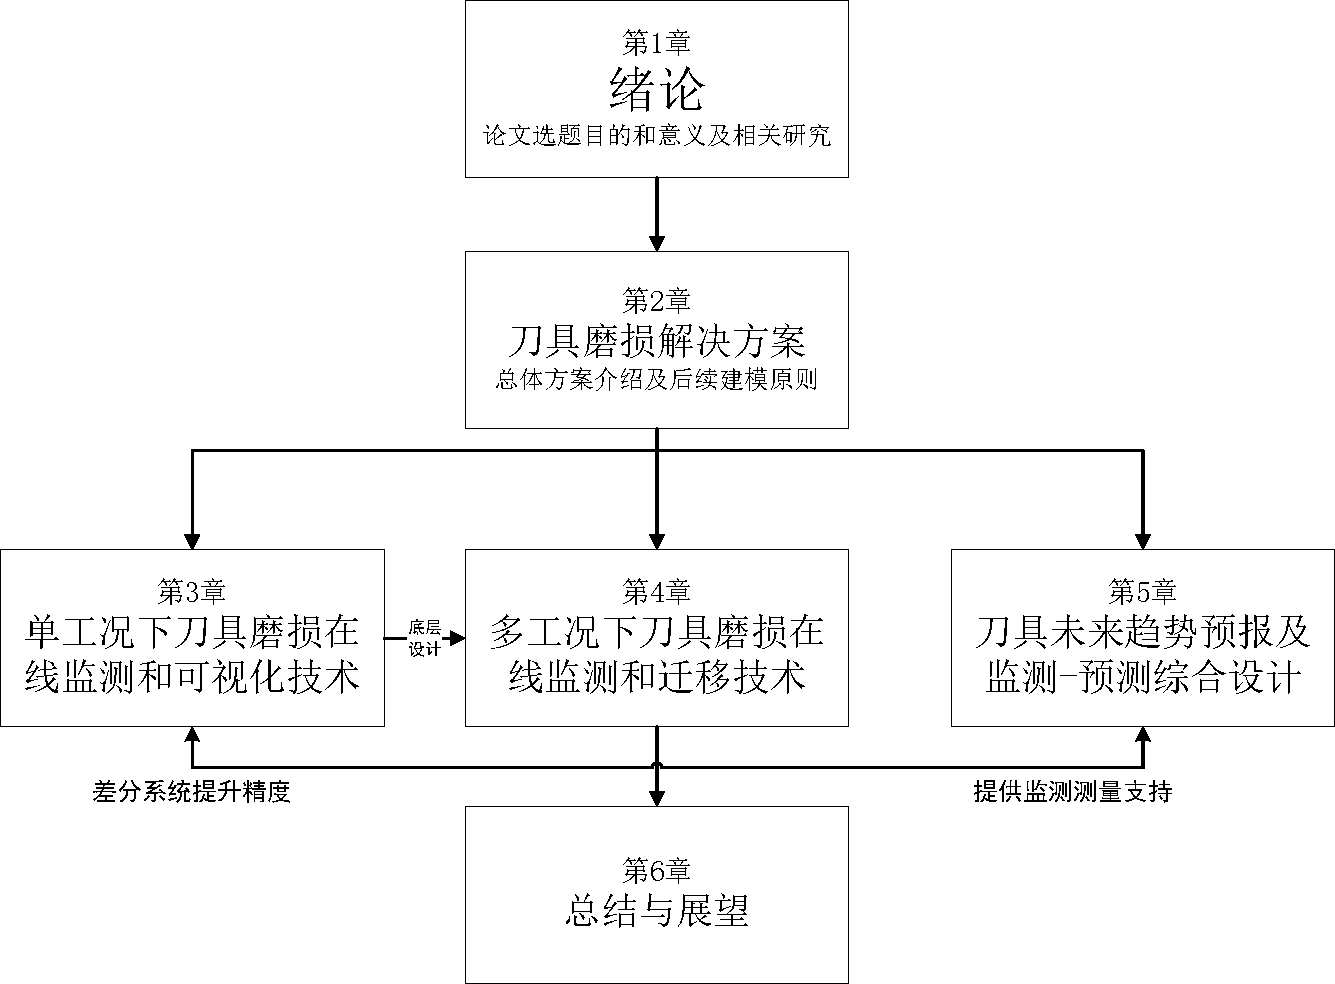
\includegraphics[width=0.7\linewidth]{figures/chapter_relation}
	\caption{各章节之间的逻辑联系}
	\label{fig:chapter_relation}
\end{figure}

\endinput



